\documentclass[letterpaper,10pt,titlepage,journal,compsoc,draftclsnofoot,onecolumn]{IEEEtran}
\newcommand\tab[1][1cm]{\hspace*{#1}}
\linespread{1}
\usepackage{graphicx}                                        
\usepackage{amssymb}                                         
\usepackage{amsmath}                                         
\usepackage{amsthm}                                          

\usepackage{alltt}                                           
\usepackage{float}
\usepackage{color}
\usepackage{url}
\usepackage{listings}

\usepackage{balance}
\usepackage[TABBOTCAP, tight]{subfigure}
\usepackage{enumitem}
\usepackage{pstricks, pst-node}

\usepackage{geometry}
\usepackage{titling}
\geometry{textheight=8.5in, textwidth=6in}


\newcommand{\cred}[1]{{\color{red}#1}}
\newcommand{\cblue}[1]{{\color{blue}#1}}

\usepackage{hyperref}
\usepackage{geometry}

\def\name{Garrett Amidon}


%% The following metadata will show up in the PDF properties
\hypersetup{
  colorlinks = true,
  urlcolor = black,
  pdfauthor = {\name},
  pdfkeywords = {cs461 ''Senior Capstone''},
  pdftitle = {CS 461 Senior Capstone: Problem Statement},
  pdfsubject = {CS461 Senior Capstone},
  pdfpagemode = UseNone
}

\title{Energy Effeciency Center Website \\
	\large Tech Review}
\author{Garrett Amidon, SR Kanna, James O'Neal}

\begin{document}
\begin{titlingpage}
    \maketitle
	\centering{}
    \begin{abstract}
        
        OSU’s Energy Efficiency Center help manufacturing and industrial companies increase their productivity and reduce their energy footprint by producing reports for energy and productivity recommendations. These reports, projects and funds are maintained in their website. The website has been developed and maintained by several programmers. As a result, the website has become disorganized, difficult to update and use. In order to remedy these issues we will design a secure, user friendly website with good code practices for the Energy Efficiency Center. 	Furthermore, the website is not accessible from mobile devices which decreases productivity while on the job site. With enough time, we would like to create a secure mobile app for the client which they are able to remotely access. This document will show the options available to fix these issues and which we think are best. 
        
    \end{abstract}
\end{titlingpage}

\newpage

\tableofcontents{}

\newpage


\section{Group Number and Name}
{Team \#36, Team WinniethePooh}

\section{Team Member Roles}

\tab{\textbf{Kanna:} Kanna will focus on the organization and the toolkit used to generate the user interface. She will also focus her efforts on web security by ensuring data remains confidential, authentic and it’s integrity. She will also create a secure login.} \newline
\tab{\textbf{James:} James will focus primarily on data visualization and code readability. Viewing and editing the projects and tasks will be one of his priorities. Providing users with the ability to view their work hours will also be his responsibility. Finally he will implement strategies for improving code readability.} \newline
\tab{\textbf{Garrett:} Garrett will focus on database management and employee records in the database to make sure that managers can view, update and create new entries. He will also implement a clock in, clock out feature so manager can keep track of what projects employees are working on and make sure they do not go over the allocated hours.} 

\section{End Goals}

\tab{We are building a secure, user friendly web application with good code practices for the Energy Efficiency Center. Stretch goals such as mobile web application or additional features will be added and evaluated based on the development process.}\newline\newline


{\textbf{Kanna:} \newline
\tab OSU’s Energy Efficiency Center help manufacturing and industrial companies increase their productivity and reduce their energy footprint by producing reports for energy and productivity recommendations. These reports, projects and funds are maintained in their website. Therefore client and employee sensitive information is maintained in the website. The website will need additional web security to ensure the data remains confidential, authentic and integrity. For example, employee and client authentication, database authentication and secure data transfer channels are all examples of secure web services we will provide.\newline\newline \tab An important subset of security is logging into the website. The website should only allow users  with clearance to access sensitive data. This prevents malicious users without authorization from accessing the information and maintains the data’s integrity. \newline\newline \tab The website has been maintained by several developers and there is a lack of usability within the website for clients and programmers. For example, the tools to maintain projects, tasks, and employees are not attractive, meeting the client's needs nor does it have continuity between them. By using the same design technology to recreate the tools, we can increase the continuity, attractiveness and ease of usability for the clients.\newline}


{\textbf{James:} \newline
\tab The primary features the client is looking to implement can be subdivided into keeping track of projects and employees. Specifically, all active employees should be listed and have account specific details such as such as pay rate, major, the date the started at the center. Specific projects should be kept track from the implementation call to the completion of the project. Projects should be marked as in-progress, complete etc. Each project should be able to add tasks noted by the task specification and task deadline. There should also be an efficient implementation for tasks not associated with a specific project, which are specific to an employee.\newline }


{\textbf{Garrett:} \newline
\tab One of the main features that will be implemented is that the website should keep record the number of hours an employee has worked on a task, specifically to keep track of task progress and to prevent employees from exceeding the maximum number of hours. Also the site needs to have pages that keep track of employees. This includes a list of all active employees as well as pages for each employee that contain information about that employee such as pay rate, major, the date the started at the center, ect… Lastly the database may need to be redone to go along with the new changes to the website. }

\section{Possible Technologies}

\subsection{Kanna:} 
\subsubsection{Security:}
\tab All softwares should be designed with security in mind. Common security risks include malicious SQL injections, forgetting to update software, XSS, error messages, server side validation, passwords, file uploads and SSL. There are some web security tools available to test a website for security. \newline\newline\tab Netsparker offers a free community and trial version. It’s main focus is to test for sql injections and XSS. Netsparker is a false positive web security scanner, meaning something which isn’t part of the system will be flagged. Netsparker is Ajax and Javascript friendly. The exploitation feature automates exploitation while the integrated exploitation conducts manual exploitation of vulnerabilities. This software is extremely easy to use and install. \newline \newline \tab OpenVas is another free software which can test for over 25000 vulnerabilities. It however is difficult to install. Extensive documentation has been provided to offset the installation and difficulty to use. Since it was the child of the closed source linux security product Nessus, it is only available in linux-like environments. OpenVas was suggested for penetration testers.\newline\newline\tab Fiddler was developed by a former Internet Security employee. Fiddler gives the user HTTP traffic by using the man-in-the-middle attack. It is a HTTP debugging proxy which intercepts, modifies, replays, compares traffic, NTLM/basic/authentication. The work is primarily done by the proxy. Fiddler is typically very easy to install and is open source. \newline
\subsubsection{Login:}
\tab Login in websites should prevent against common attacks such as sql injections, session hijacking, network eavesdropping, cross site scripting, brute force attacks,  and converting time channel attacks. \newline\newline\tab Secure login can be obtained via php and mysql. However, installing a webserver with PHP and MySQL is necessary. The database must be maintained and updated to update users and passwords, but most transactions between the server and database will be encrypted by PHP POST method. This kind of method prevents against sql injections, session hijacking, network eavesdropping, cross site scripting, brute force attacks,  and converting time channel attacks. However, it can be tedious to build and maintain.\newline\newline\tab SSL certifications, highlighted by a green url bar, show the client that their passwords and usernames will not be displayed in plaintext. The certification ensures the http will be secured against malicious attacks and can be bought. A certification is range approximately  $600 and warranty ranging at $1,500,000. SSL also address the majority of attacks login browsers should be protected against.\newline\newline\tab The third alternative is to use the canvas email. All users and employees already have secure login credentials, so the procedure will be easier to implement. However, the canvas email login is not secured against sql injections, session hijacking, network eavesdropping, cross site scripting, brute force attacks,  and converting time channel attacks.\newline
\subsubsection{UI}
\tab A key part of good human computer interaction, is user interactions. Aesthetics and ease of use are essential parts of user interactions. There are a few CSS tools which allow for a responsive website (accessible and dynamic on all platforms). \newline\newline\tab Bootstrap is an open source web application created by Twitter employees. Bootstrap offers HTML and CSS frameworks for forms, buttons, Javascript extensions, typography. Bootstrap is contained to only front-end. Although the software does not support all web browsers, it is compatible with Chrome, Firefox, IE, Opera and Safari. Bootstrap began incorporating responsive web pages and mobile-first design to increase responsiveness. The newest releases support Sass and Flexbox. Bootstrap is one of the most extensively contributed to software. \newline\newline\tab Foundation is a CSS front-end framework. Framework focuses on responsive web design by providing responsive grids, HTML/CSS templates for typography, forms, buttons, Javascript extension. Foundation is an open-source project maintained by ZURB and is primarily used by larger corporations like Facebook, Amazon, Ebay etc.\newline\newline\tab HTML5 boilerplate is an open-source web application framework. Boilerplate specializes in space conservative mobile-friendly HTML. Boilerplate provides google analytics, icons and extensive documentation. jQuery and Modernizr detection libraries are offered through Boilerplate, including Normalize.css for more CSS styles. Apache works on Boilerplate to ensure performance while server configs and ant build script are maintained through Boilerplate. \newline

\subsection{James:}
\subsubsection{Project/Tasks:}
\tab One implementation of a gantt chart can be accomplished using the third party software DHTMLX. This software is a Javascript API built for developing organizational tools. The gantt chart module has two modes, read only and editable. The creation interface is drag and drop allowing for intuitive user interaction. The chart supports projects, tasks, and milestones. Editable portions of these tasks include start time, end time, duration, completeness, and links to other projects and tasks. The gantt chart is compatible with multiple platforms including jQuery, Angularjs, and NodeJS. Additionally the gantt chart can be exported to multiple file types including PDF and PNG. This software API is a free under the GNU GPL license. \newline

%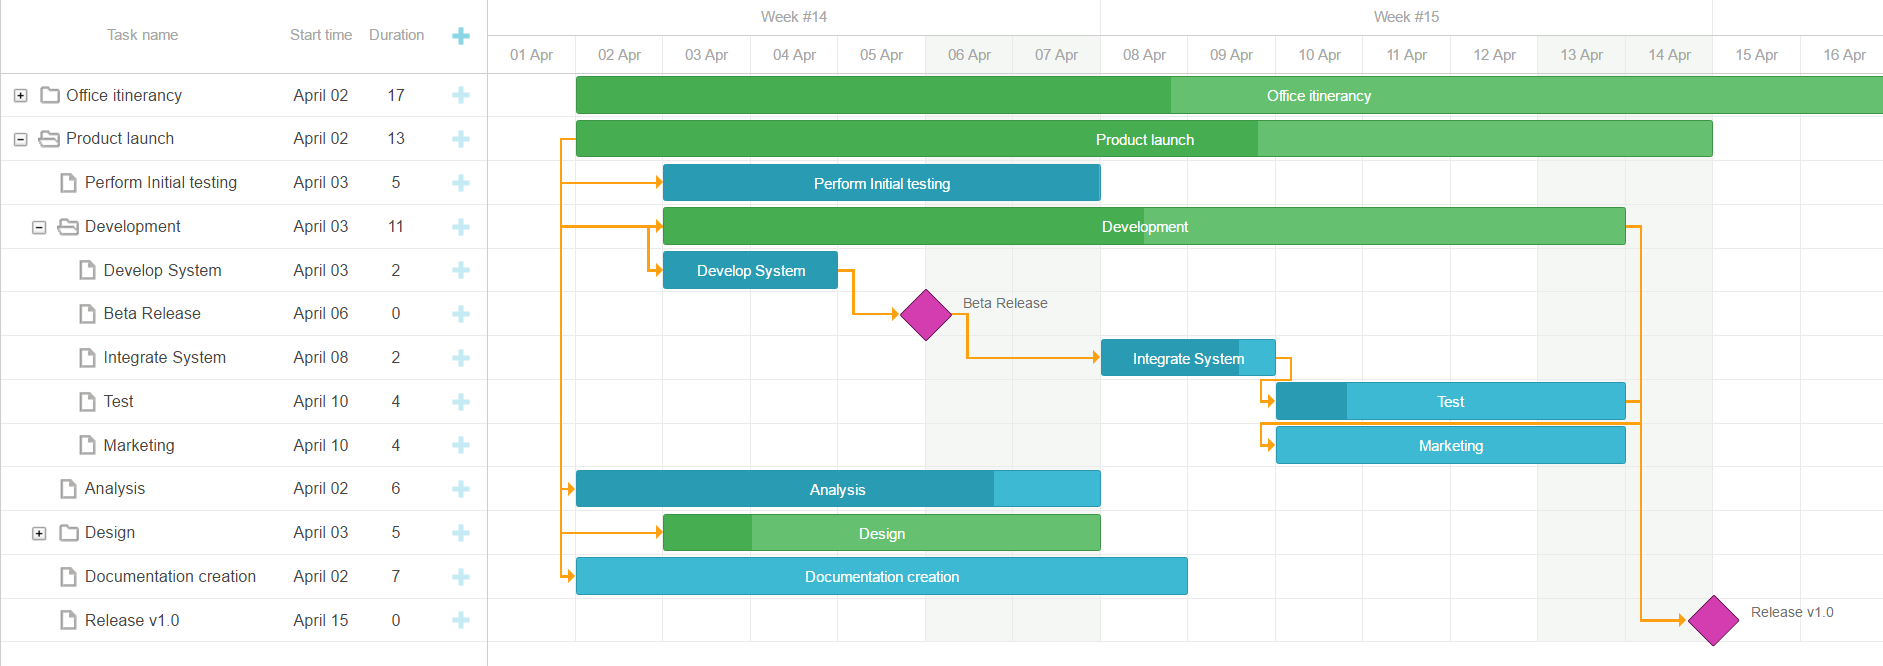
\includegraphics{James1.jpg} \newline\newline

\tab Another implementation of a gantt chart can be accomplished using D3. This is a Javascript compatible programming language for creating graphics. Creating a gantt chart in D3 requires understanding the language and designing a display. Project and task data would be pulled from the database using PHP and passed into the D3 framework for visualization. Interactive D3 charts are possible to create and are highly customizeable. The layout, colors, and size of the chart are all up to the designer. This fact makes it easy to tailor results to meet stakeholder desires. \newline

%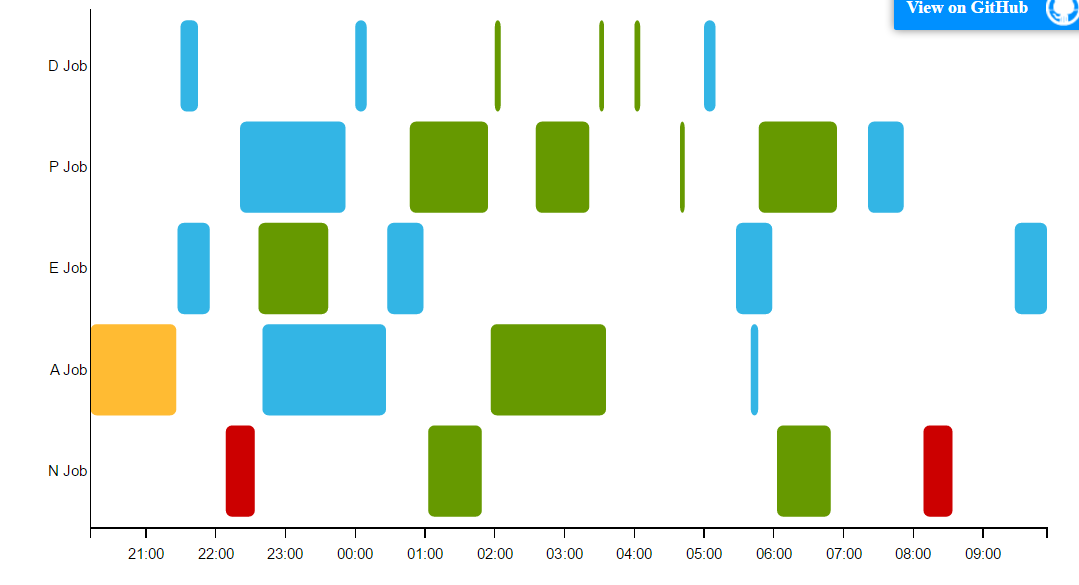
\includegraphics[scale=0.25]{James2.png} \newline\newline

\tab Alternatively, a gantt chart can be displayed using Google charts. This API designed by google runs using embedded javascript. Google charts is one of the simplest gantt chart API’s because all that is needed is the google chart libraries and a database to populate the chart. One of the most important parts of this API its integrated cross-platform and cross-browser compatability. It is fully customizable with many useful features such as grouping tasks and task dependencies. The chart is rendered using SVG which is widely used and open source. Finally, the API is very well documented providing example code and tutorials.\newline

%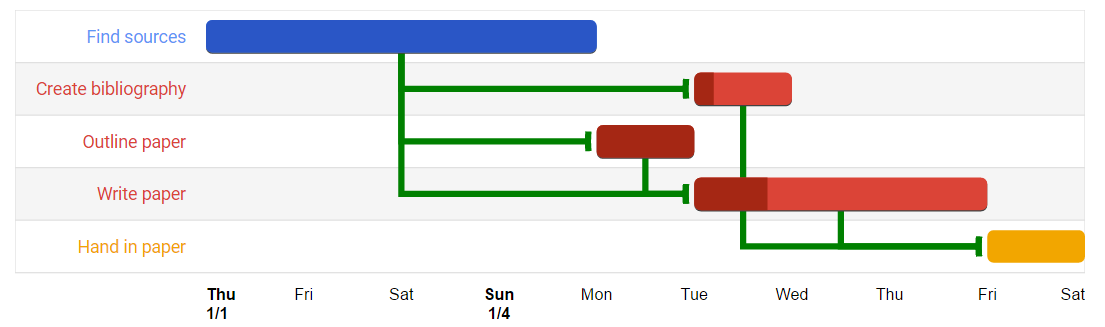
\includegraphics[scale=0.25]{James3} \newline

\subsubsection{Employee Hours}

\tab One possible implementation of an hour tracking system is HTML5. Each employee will be able to view their recorded hours in an HTML5 table. This technology also allows for editable tables making it easy for users to update where their hours have been spent. The hours can be assigned to specific tasks simply by editing a table cell. One downside to this system is it will not continually update from the database. This means that remaining hours on a task will not be updated when the user edits which task they spent time on. However, changes can still be pushed to the database and the page reloaded. \newline

%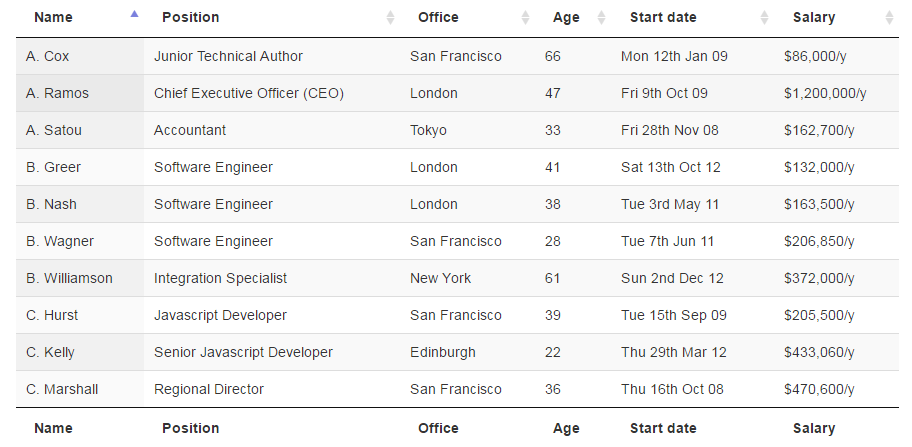
\includegraphics[scale=0.25]{James4} \newline\newline

\tab Another solution for displaying and updating work hours is a Bootstrap table. A major upside to this table is that we will already be using Bootstrap. This table also looks great and has features to hide unwanted columns and rows. This can increase simplicity and usability while also providing a clean look. This technology is a lightweight plugin which includes exporting to CSV or JSON files. This is an open source plugin which is widely supported and regularly maintained by the community. \newline

%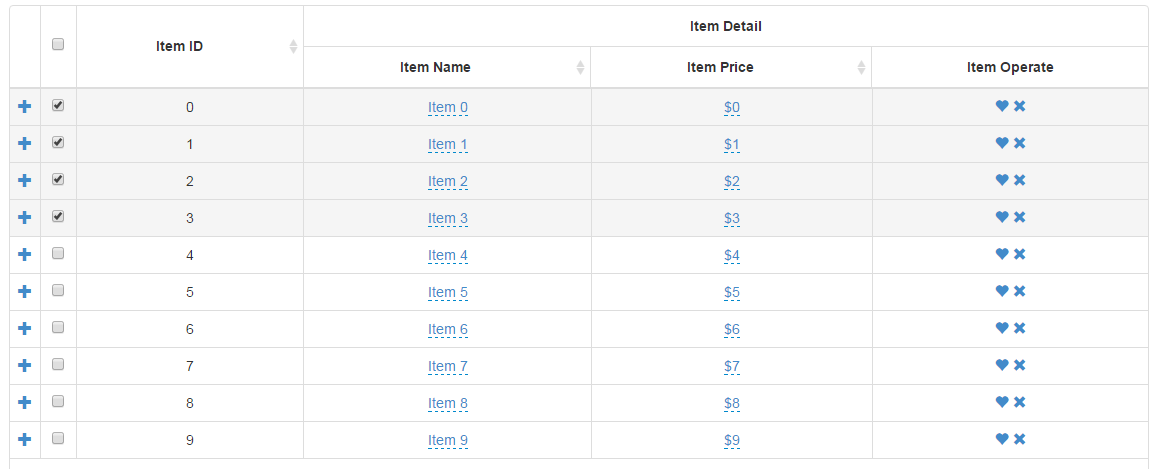
\includegraphics[scale=0.25]{James5} \newline\newline

\tab An alternative to these solutions is Tabulator. This software is a jQuery plugin which includes features such as pagination and filtering. The biggest advantage of this table is that it allows for direct table input editing. This would allow end users to update and submit data within the table allowing for quicker updates. The table accepts a wide range of data inputs including Ajax, JSON, and HTML. Unfortunately this plugin does not include customization options for its appearance. However, it has a simple design and includes graphics for added clarity. \newline

%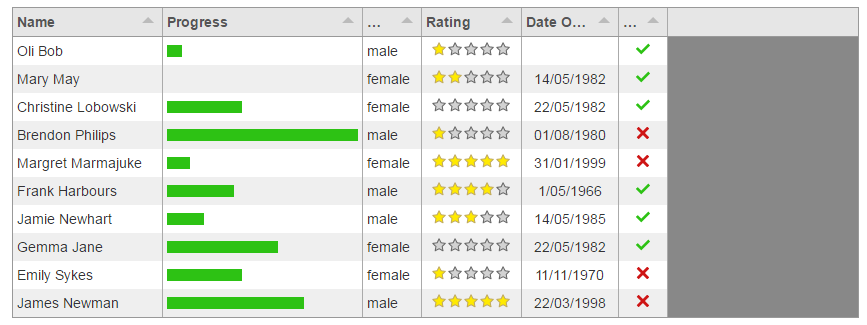
\includegraphics[scale=0.25]{James6} \newline

\subsubsection{Software Quality:}

\tab One option for measuring software quality is the ISO 9126 standard. This is an international standard for the evaluation of software. It identifies key characteristics and sub-characteristics of a software solution. The sub-characteristics are then divided into attributes. An attribute is a measurable entity within the software. By using this technique it is possible to evaluate a software solution without bias. As an example, a characteristic would be maintainability with a sub-characteristic of changeability. This would be measured by choosing a measurable attribute under the sub-characteristic of changeability and evaluating that attribute. \newline\newline\tab Another option for improving software quality is Codacy. This software is an automated code review platform. It has multiple metrics which can be turned on or off depending on the type of analyzation that needs to be done. Some of the possible metrics are accuracy, complexity, and coding style. It is compatible with multiple languages including PHP and JavaScript. It also can be integrated with GitHub making it easy to check metrics as the project progresses. In addition to its thousands of rules it also offers feedback on security and performance. Codacy is also highly secure making it viable for projects like this where data may be sensitive. \newline\newline\tab An alternative to both these solutions is using an IDE plugin. There is a plugin called sonarlint which is available in both Eclipse and Visual Studio. It works with a wide variety of code but importantly can evaluate Javascript and PHP. It includes, error checking, identification of quality issues, and hundreds of other rules to clean code. Sonarlint works constantly so mistakes and broken rules are displayed immediately. The plugin is free and widely used among developers. \newline 

\subsection{Garrett:}
\subsubsection{Employee records:}

\tab The site needs to be able to keep track of employees. The page needs to include a list of  all active employees and link to pages that contain specific employee information. This employee information contains pay rate, major, the date they started at the center as well as other information. From these pages, you must be able to view and edit employee information. To handle this request, one of the following assets can be used: database, Turbine or Excel. \newline\newline\tab A database is an organized collection of data. The data is stored and accessed through tables and queries. By having a database, the EEC will be able to make changes to employee records by using their own webpage. To do so, they will need to use web forms and “Get” and “Post” requests. These requests will be able to receive and send data to and from their database securely and as frequently with no added cost to the company. There is also many different varieties of databases available to better service the needs of the EEC. Although, databases that are on personal websites are more susceptible to attacks so employees that manage the web page will have to know about security. \newline\newline\tab Another resource that can be utilized is Turbine. Turbine is an online database company that handles all the back-end for their users. By using Turbine, users are able to manage and view employee information effortlessly without having to worry about querying, although there is a cost to use this software. The cost differs by company size; \$35 for companies with 3-20 employees, \$79 for companies with 21-50 employees, and \$159 for companies with 51-250 employees. As well as company size, the cost determines the type of support you receive. For the \$35 option, you get basic email support and online setup guides. For the \$79 option, you get priority email support, named support contact and the option to pay annually. For the most expensive option you receive priority email support, phone support, named support contact, and option to pay annually. Along with the database, every cost option receives web and mobile access so the users do not need to create their own webpage to view the database information. \newline\newline\tab One final option is to use Microsoft Excel spreadsheets. Excel is a software developed and manufactured by Microsoft Corporation that allows users to organize, format, and calculate data with formulas using a spreadsheet that is broken up by rows and columns. By using Excel, users can make changes effortlessly, without needing any knowledge of databases. There is a few drawbacks to using a spreadsheet, one of which is that the EEC will only be able to view the spreadsheet online and will have to make changes directly to the spreadsheet in order to update any information. Another is the actual cost of the software. For company use, Microsoft does not sell Excel alone, so the EEC will have to purchase the whole Office plan. The plan ranges from $8 - $35 per user a month. \newline

\subsubsection{Database:}	
\tab The current setup for the EEC that keeps track of most of the companies information, such as projects, tasks and employee information, is to use a database that is accessible through their website. This database has become cluttered and needs to be restructured. To handle this task we will use one of the following databases: SQL, MongoDB or DynamoDB. \newline\newline\tab Structured Query Language, SQL, is a standard computer language for database management. SQL is used to create queries which will insert, update and modify data. SQL is one of the most wide-used database management systems and has the added benefit of being supported across several different platforms. SQL has a lot of advantages and very few disadvantages. One advantage to SQL is that it is high speed and able to retrieve large amounts of data efficiently. This means that the EEC will be able to rely on this database to perform under high stress. The one drawback is that SQL is a commonly known language, so it is extremely susceptible to injection attacks. It also costs money to have an SQL server.\newline\newline\tab MongoDB is is an open-source, document database designed for ease of development and scaling. Since MongoDB is new and is open-source, it is constantly changing and isn’t as well known. Because of this, it may be more difficult to implement and understand. With that being said, MongoDB is available in many different versions so it can be used on a variety of different platforms. There are also many different tutorials and guides on how to use it. Also since it is open-source, it is free to use. Lastly, MongoDB allows support of both a local server and community server. Since MongoDB does not require another server to use, all data is stored in JSON format and means the database is always accessible. \newline\newline\tab DynamoDB is a fast NoSQL database made by Amazon. It is a fully managed cloud database, that also supports local use for free. This too has step by step guides on how to set up your own database and features an SQL to noSQL guide for users looking to transition. Also it is available in different programming languages, so it can be used in different software and applications. The downside to this is that to use the cloud portion, it can be expensive and as mentioned before, converting to noSQL isn’t the easiest transition. \newline

\subsubsection{Clock In/Out:}
\tab The site needs a system that allows employees to clock in and clock out for certain projects, as long as they don’t go over the amount of time allotted to that project. To handle this aspect, we will use one of the following ideas: database use, Time Clock Wizard or Open Time Clock. \newline\newline\tab With a database, when a project is posted, it will log the start date and the amount of available hours on the project. After doing so, we can create a system of clocking in to a database and then keeping track of how many hours before clocking out. When they clock in, they will be notified of how many hours are available on the project and will clock them out if they go over the posted amount. With this system it will insure that no one over works a certain project and that the company won’t be spending extra time on projects. Also, if the manager decides to change the amount of time on a project, this can easily be done so in the database. \newline\newline\tab Another option is to use the Time Clock Wizard. The time clock wizard is an online service the handles clocking in and out. When an employee clocks in, there is a designated phone number that Time Clock Wizard will text to notify that someone has logged in. From there the manager can keep track of who has clocked into what projects and notify employees when they are about to go over the allotted amount. Unfortunately, the service will not automatically keep track of how many hours the project has and automatically notify employees, this is the main drawback besides the cost of using the program. \newline\newline\tab One final option is to use Open Time Clock. Open Time Clock is similar to Time Clock Wizard, but does notify the manager when someone clocks in. Instead, this program focuses more on security to make sure someone isn’t clocking in for a co-worker. A feature that this program has that Time Clock Wizard doesn’t is photo confirmation. This program will take a photo and compare it to a previous photo to make sure it is actually the correct employee logging in. This program can either be free or purchased, giving extra features with the purchased version. \newline

\section{Decided Technologies}

\subsection{Kanna:}
\subsubsection{Security:}
\tab As mentioned above, security should be designed alongside the software. Threats to consider and our criteria for evaluation include malicious SQL injections, forgetting to update software, XSS, error messages, server side validation, passwords, file uploads and SSL among others. All of the security scanning software being considered is open-source, so price is not an issue. Netsparker addresses sql injection and XSS, but fails to focus the other main security threats. Netsparker is noted for it’s ease of use. OpenVas is the most extensive of the three security scanning options, since it can test over 25000 vulnerabilities. However, it’s difficulty to use and time consumption is notorious. Fiddler focuses on vulnerabilities in HTTP traffic, which does not address any criteria except authenticity. I would like to suggest using OpenVas for the most rigorous security scanning model and meets the most criteria, but to note that if it’s too difficult and time-consuming to use, then Netsparker will be supplemented to the scanning process. \newline

\subsubsection{Login:}
\tab Login in websites should prevent against common attacks such as sql injections, session hijacking, network eavesdropping, cross site scripting, brute force attacks,  and converting time channel attacks. The best method to prevent against these attacks is a combination of secure login can be obtained via php and mysql. This kind of method prevents against sql injections, session hijacking, network eavesdropping, cross site scripting, brute force attacks,  and converting time channel attacks. Furthermore, since I am experienced with sql and php, there would be a minimal learning curve and time wasted. Even though it can be tedious to build and maintain, it can be combined with the canvas email structure so users do not have create a second email. \newline

\subsubsection{UI:}
\tab Users expect aesthetics and ease of use when interacting with web applications. CSS tools like Bootstrap, Foundation and Boilerplate provide structure, navigation and aesthetic appeal on all web platforms. All three are responsive web tools and all three provide HTML and CSS frameworks for forms, buttons, Javascript extensions, typography. Bootstrap and Foundation’s offerings are more extensive that Boilerplate’s. All three are supported by multiple browsers, but Bootstrap and Foundation are the most extensive. However, Boilerplate is the most lightweight platform option. Bootstrap has a large open-source platform and is geared towards engineers to use and contribute to. Foundation is primarily used by large corporations. I am also extremely familiar with Bootstrap, so there would be a minimal learning curve or time wasted. Under the categories of structure, aesthetics, time and responsiveness, I recommend using Bootstrap. \newline	

\subsection{James:}
\subsubsection{Projects and Tasks:}
\tab Projects and tasks are vital to the operation and organization of the EEC. In order to stay on track and be productive employees need to keep track of projects and tasks. Additionally they need a clear view of project timelines and status of specific tasks. All this information needs to be easily viewable and readily available. The best technology to implement a solution is DHTMLX. The API looks great and has highly customizable features. It is excellently documented and includes tutorials and examples. It includes drag and drop functionality giving it high usability. It automatically updates the database with any changes made with the chartt. This feature can also be turned off so only certain individuals can make changes to project information using the chart. Overall this API is better than the others because it is simple to implement, use, and modify. \newline

\subsubsection{Employee Hours:}
\tab Displaying employee hours is important for the employees and their supervisor. They need clear visuals that allow them to verify correct inputs. Additionally they will not want a complex or time consuming process for managing and updating their hours. To accomplish this the best technology to use is Tabulator. With tabulator the table view of hours is consistent and easy to read. It supports organization and pagination features which will make finding specific rows easy. Interactive editing will allow users to quickly update and manage their hours. Tabulator’s documentation, features, and ease of use put it ahead of the other options. \newline

\subsubsection{Software Quality:}
\tab Software quality is important for the website because we will not be maintaining it in the future. Employees of the company will need to take what we have built and understand it well enough to make changes. While code standards and metrics will be used while writing it a software tool could greatly increase our successfulness in meeting this requirement. We will be implementing Codacy into our final solution. This software provides endless rules to check our final code with. It also will not reduce productivity because it can be integrated straight into github. The best part about Codacy is its professional quality and ability to catch errors from start to finish. \newline

\subsection{Garrett:}
\subsubsection{Employee records:}
\tab Employee records are private and need to be accessed on the daily, so having your own database ensures no one else has access to these records and will always be available. By using a web page and forms to submit changes to your database, you are in control of security and can be used at your disposal. By using Turbine to manage your employee records, you are putting your records at risk because security is out of your hands. Also, if Turbine’s servers are ever down, you cannot access your employee records. With regards to Excel, having to open the spreadsheet to make changes is not the most optimal process. Also, if the spreadsheet gets large, it will start to slow down when you open the document to make changes. The database route ensures that the user will get the most reliable and efficient results.  \newline 

\subsubsection{Database:}
\tab For the database type, going with SQL is the best. Because of its wide-use, the EEC already has an SQL server implemented. Considering there is no big drawbacks to using SQL, it seems unnecessary to force a company to learn something new. Also with SQL you can access your tables through MySQL, so you do not need to know how to query to select results or view database entries. Plus, if you do need to create a query, by using MySQL it will create the query for you and give you the code to use in your webpage. Overall, SQL will provide the best service and overall best experience for the EEC. \newline

\subsubsection{Clock In/Out:}
\tab Again, the best way to handle this system is through database handling. The named time clocks are great for keeping track of when someone clocks in and out, but not for when someone goes over hours on a certain project. With a database, we can store when a project is started and how much time it can be worked on. After doing so, when an employee goes to clock in, it can notify them the available hours left on that project and won’t allow them to go past the posted amount. \newline




\end{document}
